\section{Results}
\label{sec:results}

We present results through the three lenses in turn---objective novelty (\secref{sec:res_lgn}), the judge rubric and pairwise comparisons (\secref{sec:res_judge}), set-level diversity (\secref{sec:res_div})---and close with the judge-validation test that ties them together (\secref{sec:res_valid}). The headline is that the lenses \emph{disagree}, in a way that is itself the main finding.

\subsection{Objective literature-grounded novelty: no grounding helps}
\label{sec:res_lgn}

\Tabref{tab:lgn} reports \lgn relative to the unguided control. \emph{No grounding mechanism significantly increases objective novelty.} The only Holm-significant effect is in the wrong direction: \proposal makes ideas \emph{more} conventional---closer to existing work---than the control ($d = -0.66$, Holm $p = 0.007$). \induction and \outcome trend the same way ($d = -0.40$ and $-0.34$) but do not survive correction. \deduction and \litcomp, the two conditions that most raise \emph{judged} novelty (\secref{sec:res_judge}), are statistically indistinguishable from the control on \lgn ($d = 0.09$ and $0.01$). H1 is refuted: grounding does not move ideas farther from real prior work, and one mechanism pulls them closer. \Figref{fig:lgn} shows the same picture.

\begin{table}[t]
    \centering
    \caption{Objective literature-grounded novelty (\lgn) by condition, from the mixed-effects model with \unguided as reference. Higher \lgn means more distant from real prior work. Effects are robust to a length covariate (rightmost column). The only Holm-significant effect makes ideas \emph{less} novel. Best (most novel) grounded value in \textbf{bold}; the significant effect is marked \checkmark.}
    \label{tab:lgn}
    \begin{tabular}{@{}lccccc@{}}
        \toprule
        Condition & \lgn mean & Cohen's $d$ & $p$ & Holm $p$ & $p$ (len.\ cov.) \\
        \midrule
        \unguided (control)   & 0.188 & ---    & ---   & ---   & ---   \\
        \midrule
        \deduction            & \textbf{0.190} & $+0.09$ & 0.678 & 1.000 & 0.687 \\
        \litcomp              & 0.188 & $+0.01$ & 0.971 & 1.000 & 0.984 \\
        \smallexp             & 0.181 & $-0.19$ & 0.334 & 1.000 & 0.393 \\
        \outcome              & 0.176 & $-0.34$ & 0.089 & 0.358 & 0.090 \\
        \induction            & 0.174 & $-0.40$ & 0.044 & 0.219 & 0.045 \\
        \proposal             & 0.165 & $-0.66$ & 0.001 & \textbf{0.007}~\checkmark & 0.001 \\
        \bottomrule
    \end{tabular}
\end{table}

\begin{figure}[t]
    \centering
    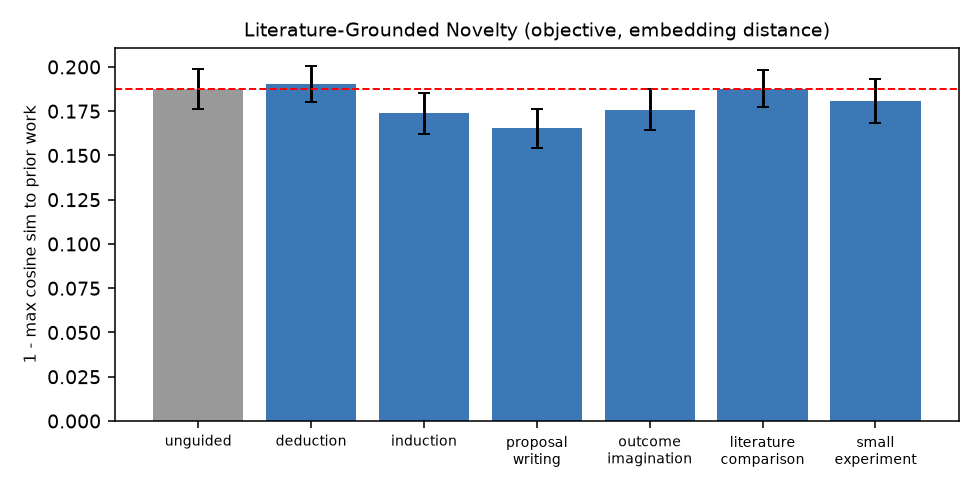
\includegraphics[width=0.62\linewidth]{figures/fig1_lgn.png}
    \caption{Objective literature-grounded novelty (\lgn) by condition, with the unguided control marked. No grounding mechanism rises above the control; \proposal sits significantly below it. Grounding does not increase genuine distance from prior work.}
    \label{fig:lgn}
\end{figure}

\subsection{Judge rubric and pairwise comparisons: a steered trade-off}
\label{sec:res_judge}

The LLM judges tell a very different story (\Tabref{tab:rubric}). On \emph{judged} novelty, \deduction is the clear winner ($5.94$ vs.\ $5.49$, $d = +0.81$, Holm-significant), with \litcomp and \outcome also up ($d = +0.57$ and $+0.59$). But these gains come with a feasibility cost. The conditions split into two clean clusters. \emph{Generative} grounding (\deduction, \litcomp, \outcome) raises judged novelty but lowers feasibility; \emph{validation} grounding (\smallexp, \induction, \proposal) raises feasibility but leaves novelty flat or lower. \smallexp is the extreme case: it has the highest feasibility ($7.84$, $d = +0.77$) but the lowest novelty ($5.17$, $d = -0.64$) and the only Holm-significant drop in \emph{overall} score ($5.11$, $d = -0.91$). No condition beats the control on overall quality. \Figref{fig:rubric} and the trade-off view in \Figref{fig:tradeoff} make the two clusters visible. H2 is only partially supported (judged novelty, for 2--3 mechanisms), and H3's trade-off is confirmed.

\begin{table}[t]
    \centering
    \caption{Judge rubric scores (1--10, mean over both judges) by condition. \checkmark marks a Holm-significant gain and {\footnotesize\textsf{X}} a Holm-significant loss versus the control. Generative grounding (top group) raises novelty but lowers feasibility; validation grounding (bottom group) does the reverse. No condition improves overall quality, and \smallexp significantly worsens it.}
    \label{tab:rubric}
    \begin{tabular}{@{}lccc@{}}
        \toprule
        Condition & Novelty & Feasibility & Overall \\
        \midrule
        \unguided               & 5.49 & 7.20 & 5.44 \\
        \midrule
        \deduction              & \textbf{5.94}~\checkmark {\scriptsize($d{=}{+}0.81$)} & 6.91 & 5.44 \\
        \litcomp                & 5.80 {\scriptsize($d{=}{+}0.57$)} & 6.83 & 5.36 \\
        \outcome                & 5.70 {\scriptsize($d{=}{+}0.59$)} & 6.89 & 5.46 \\
        \midrule
        \induction              & 5.49 & 7.69 {\scriptsize($d{=}{+}0.59$)} & 5.47 \\
        \proposal               & 5.43 & 7.67 {\scriptsize($d{=}{+}0.54$)} & 5.33 \\
        \smallexp               & 5.17 {\scriptsize($d{=}{-}0.64$)} & \textbf{7.84}~\checkmark {\scriptsize($d{=}{+}0.77$)} & 5.11~{\footnotesize\textsf{X}} {\scriptsize($d{=}{-}0.91$)} \\
        \bottomrule
    \end{tabular}
\end{table}

\begin{figure}[t]
    \centering
    \begin{subfigure}[b]{0.48\textwidth}
        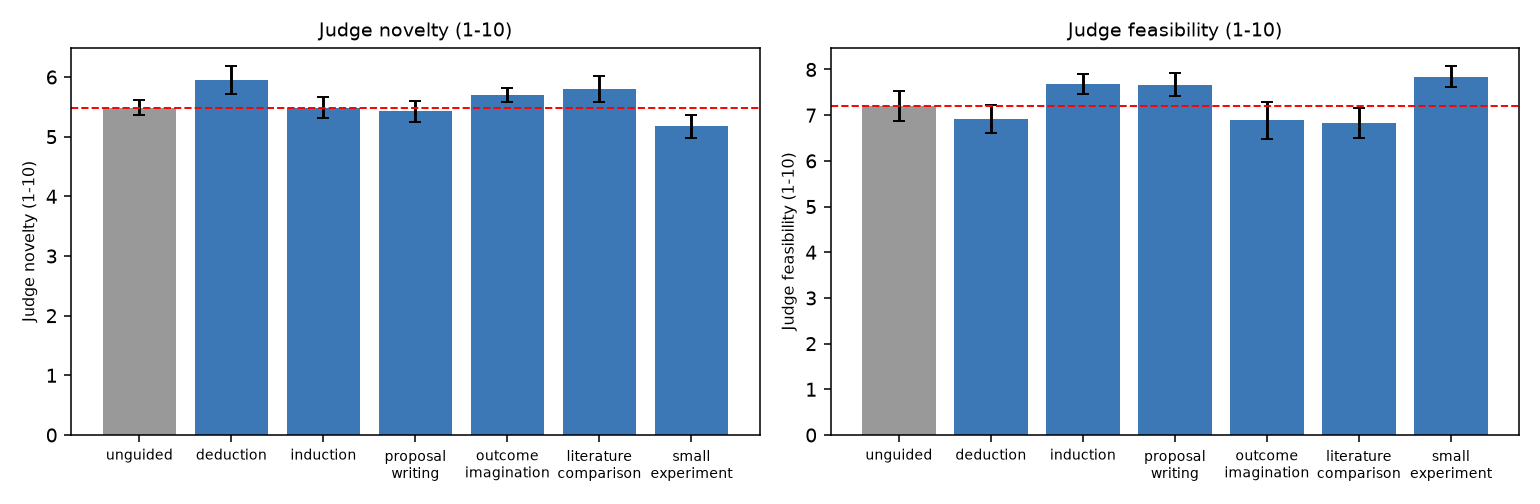
\includegraphics[width=\textwidth]{figures/fig2_judge_rubric.png}
        \caption{Rubric scores by condition}
        \label{fig:rubric}
    \end{subfigure}
    \hfill
    \begin{subfigure}[b]{0.48\textwidth}
        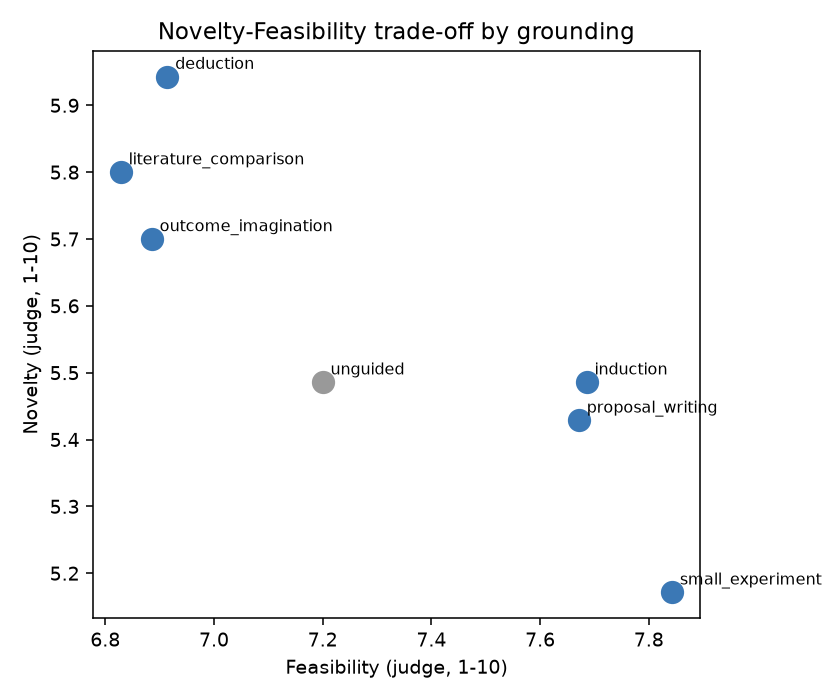
\includegraphics[width=\textwidth]{figures/fig3_tradeoff.png}
        \caption{Novelty--feasibility trade-off}
        \label{fig:tradeoff}
    \end{subfigure}
    \caption{Judge rubric results. \captiona Mean rubric scores by condition. \captionb Each condition placed on the novelty--feasibility plane relative to the control: generative grounding moves up-left (more novel, less feasible), validation grounding moves down-right (less novel, more feasible). Grounding is a steering knob, not a uniform quality lever.}
    \label{fig:judge}
\end{figure}

\para{Pairwise win-rate.} Pairwise judging is more sensitive than absolute scoring (\Tabref{tab:pairwise}, \Figref{fig:pairwise}). \litcomp is preferred over the control $79\%$ of the time ($p < 0.001$) even though its \emph{absolute} overall score was flat---a known absolute-versus-comparative judging gap. \outcome ($65\%$) and \deduction ($62\%$) also win significantly. At the other end, \smallexp is reliably \emph{dis-preferred} ($33\%$, $p = 0.005$), consistent with its low novelty and overall scores.

\begin{table}[t]
    \centering
    \caption{Pairwise win-rate $P(\text{grounded} \succ \unguided)$ on overall preference, position-controlled across 2 judges $\times$ 2 orderings ($n = 35$ per condition). \checkmark marks a significant win, {\footnotesize\textsf{X}} a significant loss, versus chance (0.5). Best in \textbf{bold}.}
    \label{tab:pairwise}
    \begin{tabular}{@{}lccc@{}}
        \toprule
        Condition & Win-rate & 95\% CI & $p$ vs.\ 0.5 \\
        \midrule
        \litcomp        & \textbf{0.79} & [0.71, 0.86] & $<0.001$~\checkmark \\
        \outcome        & 0.65 & [0.55, 0.74] & 0.006~\checkmark \\
        \deduction      & 0.62 & [0.51, 0.72] & 0.033~\checkmark \\
        \induction      & 0.46 & [0.37, 0.56] & 0.468 \\
        \proposal       & 0.43 & [0.33, 0.53] & 0.177 \\
        \smallexp       & 0.33 & [0.22, 0.44] & 0.005~{\footnotesize\textsf{X}} \\
        \bottomrule
    \end{tabular}
\end{table}

\begin{figure}[t]
    \centering
    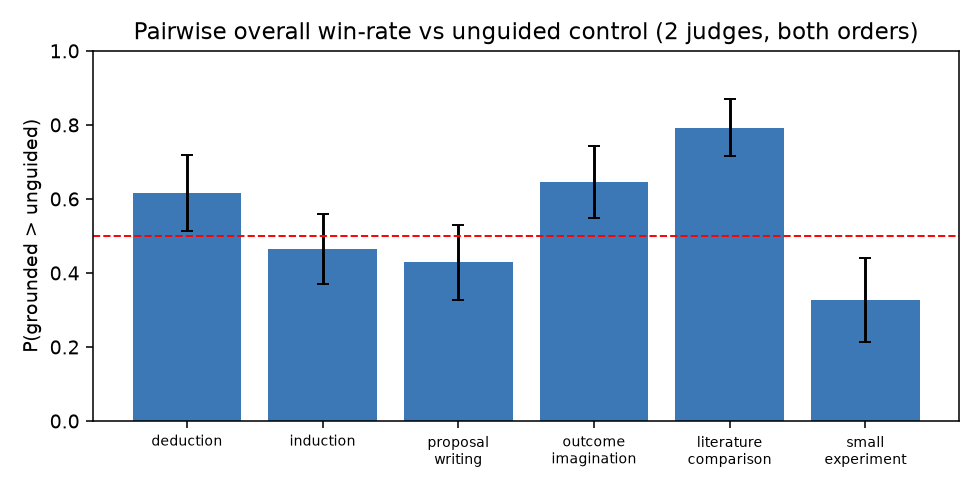
\includegraphics[width=0.62\linewidth]{figures/fig4_pairwise.png}
    \caption{Pairwise overall win-rate against the unguided control with bootstrap 95\% CIs; the dashed line marks chance (0.5). \litcomp wins $79\%$ of comparisons; \smallexp is reliably dis-preferred.}
    \label{fig:pairwise}
\end{figure}

\subsection{Set-level diversity}
\label{sec:res_div}

\Tabref{tab:diversity} reports within-cell diversity. Only \litcomp meaningfully increases mean pairwise distance ($0.456$ vs.\ $0.412$) while lowering the near-duplicate rate ($0.091$ vs.\ $0.106$), consistent with its retrieve-and-differentiate mechanism. The other conditions are at or slightly below the control. H4 is supported only for literature comparison; grounding does not broadly fix the diversity collapse documented by \citet{si2024can}. \Figref{fig:diversity} visualizes the ranking.

\begin{table}[t]
    \centering
    \caption{Set-level diversity within (condition $\times$ topic) cells. Higher mean pairwise distance and lower near-duplicate rate (cosine $\geq 0.8$) are better. Only \litcomp improves on the control for both. Best in \textbf{bold}.}
    \label{tab:diversity}
    \begin{tabular}{@{}lcc@{}}
        \toprule
        Condition & Mean pairwise dist.\ $\uparrow$ & Near-dup rate $\downarrow$ \\
        \midrule
        \litcomp        & \textbf{0.456} & \textbf{0.091} \\
        \smallexp       & 0.424 & 0.094 \\
        \unguided       & 0.412 & 0.106 \\
        \outcome        & 0.407 & 0.096 \\
        \deduction      & 0.404 & 0.104 \\
        \proposal       & 0.397 & 0.109 \\
        \induction      & 0.393 & 0.106 \\
        \bottomrule
    \end{tabular}
\end{table}

\begin{figure}[t]
    \centering
    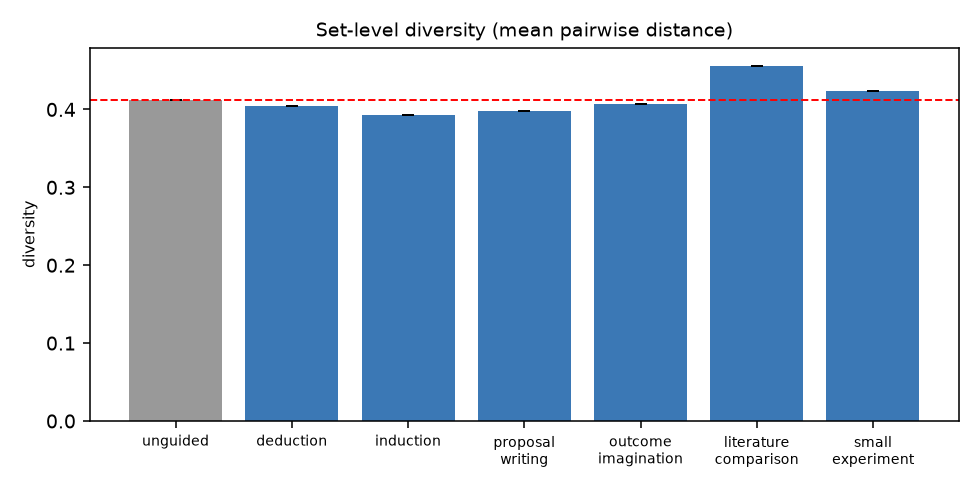
\includegraphics[width=0.6\linewidth]{figures/fig5_diversity.png}
    \caption{Mean within-cell pairwise distance by condition. Only \litcomp clearly exceeds the unguided control, matching its retrieve-and-differentiate design.}
    \label{fig:diversity}
\end{figure}

\subsection{Judge validation: the novelty mirage, measured}
\label{sec:res_valid}

The three lenses can only be reconciled by checking whether the judge measures what \lgn measures. It does not. The two judges \emph{agree with each other}: their novelty scores correlate at Spearman $\rho = 0.41$ ($p = 8 \times 10^{-11}$), moderate and significant, so the rubric is reliable enough to interpret. But judge novelty and objective \lgn are \emph{unrelated}: Spearman $\rho = 0.012$ ($p = 0.85$), essentially zero (\Figref{fig:convergent}). H5 is refuted. This is the crux: the judges reliably reward something, and that something is \emph{not} distance from prior work. The novelty gains in \secref{sec:res_judge} are real in the judges' shared eye and a mirage under a literature-anchored measure---a controlled, item-level reproduction of the novelty mirage~\citep{rqbench2026}.

\begin{figure}[t]
    \centering
    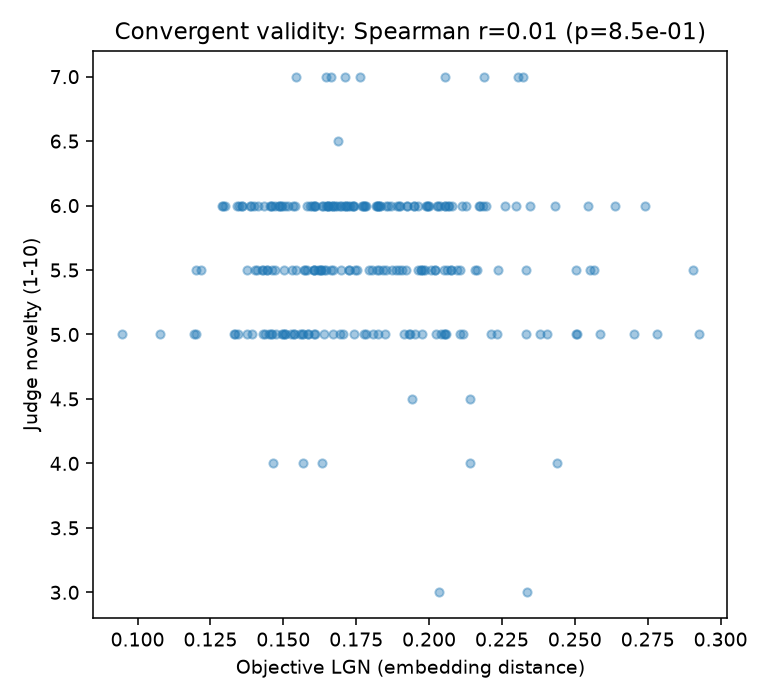
\includegraphics[width=0.6\linewidth]{figures/fig6_convergent.png}
    \caption{Convergent-validity scatter: mean judge novelty (1--10) versus objective \lgn at the item level. The flat trend (Spearman $\rho = 0.01$, $p = 0.85$) shows the two are uncorrelated, even though the two judges agree with each other ($\rho = 0.41$). LLM-judged novelty and literature-distance novelty are different constructs.}
    \label{fig:convergent}
\end{figure}
